\documentclass[11pt,a4paper]{article}

\usepackage[margin=1in]{geometry}
\usepackage{amsmath,amssymb,bm,mathtools}
\usepackage{booktabs,longtable,array,tabularx,multirow}
\usepackage{enumitem}
\usepackage{xcolor}
\usepackage{hyperref}
\usepackage{graphicx}
\usepackage{microtype}
\usepackage{fancyhdr}
\usepackage{titlesec}
\usepackage{listings}
\usepackage{tikz}
\usetikzlibrary{arrows.meta,positioning,shapes.geometric,fit}

\definecolor{navy}{RGB}{25,55,95}
\definecolor{lightblue}{RGB}{235,243,252}
\definecolor{lightgray}{RGB}{246,246,246}
\definecolor{darkgray}{RGB}{70,70,70}

\hypersetup{
  colorlinks=true,
  linkcolor=navy,
  urlcolor=navy,
  citecolor=navy,
  pdftitle={A Four-Layer Framework for Understanding Medical Image Registration},
  pdfauthor={Cao Pham Minh Dang}
}

\pagestyle{fancy}
\fancyhf{}
\lhead{Medical Image Registration}
\rhead{Four-Layer Framework}
\cfoot{\thepage}
\setlength{\headheight}{14pt}

\titleformat{\section}{\Large\bfseries\color{navy}}{\thesection}{0.7em}{}
\titleformat{\subsection}{\large\bfseries\color{navy}}{\thesubsection}{0.7em}{}
\titleformat{\subsubsection}{\normalsize\bfseries}{\thesubsubsection}{0.7em}{}

\setlist[itemize]{leftmargin=1.6em}
\setlist[enumerate]{leftmargin=1.8em}
\renewcommand{\arraystretch}{1.2}

\newcommand{\R}{\mathbb{R}}
\newcommand{\T}{\mathcal{T}}
\newcommand{\Loss}{\mathcal{L}}
\newcommand{\fixed}{I_F}
\newcommand{\moving}{I_M}
\newcommand{\sdf}{\operatorname{SDF}}
\newcommand{\argmin}{\operatorname*{arg\,min}}

\begin{document}

\begin{titlepage}
\centering
\vspace*{2.5cm}
{\Huge\bfseries A Four-Layer Framework for Understanding Medical Image Registration\par}
\vspace{0.6cm}
{\Large From Rigid Motion and ICP to SDFs, B-Splines, and Diffeomorphic Registration\par}
\vspace{1.5cm}
{\large Cao Pham Minh Dang\par}
\vfill
\begin{minipage}{0.88\textwidth}
\small
\textbf{Purpose.} This note organizes image registration into four conceptual layers: \emph{representation / registration signal}, \emph{transformation model}, \emph{matching objective / metric}, and \emph{optimizer / solver}. The goal is to make apparently different terms---such as intensity-based registration, SDF registration, ICP, rigid transforms, affine transforms, B-splines, mutual information, and L-BFGS---fit into one coherent mental model.
\end{minipage}
\vspace{1.5cm}
\end{titlepage}

\tableofcontents
\newpage

\section{What Is Image Registration?}

Image registration estimates a spatial transformation that brings a \emph{moving} image or geometry into alignment with a \emph{fixed} image or geometry.

Let
\[
\fixed : \Omega_F \to \R,
\qquad
\moving : \Omega_M \to \R
\]
be fixed and moving images. A transformation
\[
\T_{\theta}: \Omega_M \to \Omega_F
\]
with parameters $\theta$ maps coordinates from the moving domain to the fixed domain.

The abstract registration problem is
\[
\boxed{
\theta^*
=
\argmin_{\theta}
\Loss\bigl(F,\,M\circ \T_{\theta}^{-1}\bigr)
}
\]
where $F$ and $M$ need not be raw images: they may be intensities, masks, signed-distance fields, landmarks, point clouds, or learned features.

The central difficulty is that words commonly used in registration literature belong to \emph{different conceptual levels}. For example:

\begin{itemize}
  \item \textbf{SDF} describes a representation of a segmentation.
  \item \textbf{Rigid, affine, B-spline, diffeomorphic} describe transformation models.
  \item \textbf{Dice, NCC, mutual information, Chamfer distance} describe objectives or similarity measures.
  \item \textbf{Adam, L-BFGS, Powell, SVD} describe optimization or solution strategies.
  \item \textbf{ICP} is not simply one of the above; it is an algorithmic framework that combines correspondence estimation, an objective, and an iterative solver.
\end{itemize}

This motivates the four-layer framework used throughout this document.

\section{The Four-Layer Mental Model}

A useful way to understand almost any registration method is to ask four questions in order:

\begin{center}
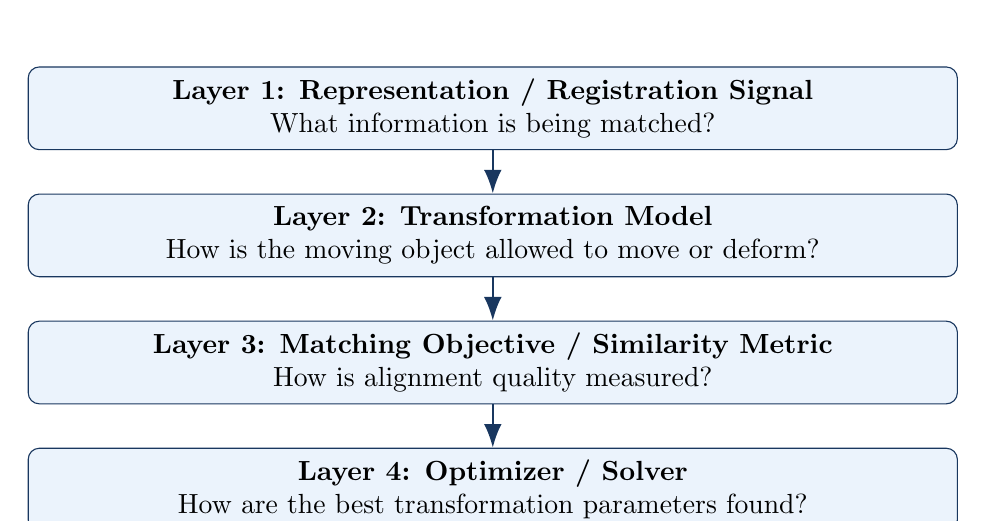
\begin{tikzpicture}[
  node distance=0.55cm,
  box/.style={draw=navy, rounded corners, fill=lightblue, minimum width=11.8cm, minimum height=1.05cm, align=center},
  arr/.style={-{Latex[length=3mm]}, thick, navy}
]
\node[box] (a) {\textbf{Layer 1: Representation / Registration Signal}\\What information is being matched?};
\node[box, below=of a] (b) {\textbf{Layer 2: Transformation Model}\\How is the moving object allowed to move or deform?};
\node[box, below=of b] (c) {\textbf{Layer 3: Matching Objective / Similarity Metric}\\How is alignment quality measured?};
\node[box, below=of c] (d) {\textbf{Layer 4: Optimizer / Solver}\\How are the best transformation parameters found?};
\draw[arr] (a) -- (b);
\draw[arr] (b) -- (c);
\draw[arr] (c) -- (d);
\end{tikzpicture}
\end{center}

In compact form:
\[
\boxed{
\text{Representation}
\rightarrow
\text{Transformation}
\rightarrow
\text{Objective}
\rightarrow
\text{Optimizer}
}
\]

A registration method can therefore be specified as a tuple:
\[
\boxed{
(\text{signal},\ \text{transform},\ \text{metric},\ \text{solver})
}
\]

For example:
\[
(\text{multi-label SDF},\ \text{rigid},\ \text{SDF loss},\ \text{L-BFGS})
\]
or
\[
(\text{surface points},\ \text{rigid},\ \text{nearest-point distance},\ \text{ICP/SVD}).
\]

\section{Layer 1: Representation / Registration Signal}

Layer 1 answers:

\begin{quote}
\textbf{What information from the fixed and moving data is actually used to establish alignment?}
\end{quote}

\subsection{Intensity-Based Registration}

Intensity-based methods operate directly on voxel or pixel values. The registration signal is therefore
\[
F(x)=I_F(x),
\qquad
M(x)=I_M(x).
\]

Typical applications include CT--CT, MRI--MRI, PET--CT, and sometimes CT--MRI or CT--US if a suitable multimodal metric is used.

For a transformed moving image,
\[
I_M^T(x)=I_M\bigl(T^{-1}(x)\bigr),
\]
registration compares $I_F(x)$ with $I_M^T(x)$ over a region of interest.

Intensity-based registration is attractive because it does not require segmentation or landmark extraction. However, it can be difficult in multimodal settings because intensities do not necessarily have the same physical meaning across modalities.

\subsection{Feature-Based Registration}

Feature-based registration first extracts a representation
\[
f(I)
\]
from each image and registers those features instead of raw intensity.

Examples include:
\begin{itemize}
  \item anatomical landmarks,
  \item keypoints,
  \item edges and contours,
  \item vessel bifurcations,
  \item surfaces,
  \item segmentation masks,
  \item signed-distance fields,
  \item learned feature maps from neural networks.
\end{itemize}

A common conceptual hierarchy is
\[
\boxed{
\text{Registration signal}
\in
\{\text{intensity-based},\ \text{feature/geometry-based}\}
}
\]
with segmentation-based, landmark-based, and surface-based registration often treated as subclasses of feature-based registration. Terminology varies across papers, so segmentation-based methods are sometimes presented as a separate category.

\subsection{Segmentation Masks}

A binary segmentation mask is
\[
M(x)\in\{0,1\}.
\]
For a multi-label problem, one can use
\[
M_c(x)\in\{0,1\},
\qquad c\in\mathcal{C},
\]
where $\mathcal{C}$ might contain structures such as LV, RV, LA, RA, and myocardium.

Registration can then directly optimize a mask-based objective such as Dice, or convert masks into smoother geometric representations such as SDFs.

\subsection{Signed-Distance Fields (SDFs)}

Given a segmented region $\Omega$ with boundary $\partial\Omega$, a signed-distance field is commonly defined as
\[
\phi(x)=\sdf(x)=
\begin{cases}
-d(x,\partial\Omega), & x\in\Omega,\\
0, & x\in\partial\Omega,\\
+d(x,\partial\Omega), & x\notin\Omega,
\end{cases}
\]
where
\[
d(x,\partial\Omega)=\min_{y\in\partial\Omega}\|x-y\|_2.
\]

The sign convention may be reversed in some libraries, but the geometric idea is the same: every point stores its distance to the surface.

Compared with a binary mask, the SDF gives a spatially smooth signal around the boundary. Even if two masks do not overlap, their distance fields can still provide a useful optimization signal.

A clipped and normalized SDF can be written as
\[
\tilde\phi(x)
=
\frac{\operatorname{clip}(\phi(x),-d_{\max},d_{\max})}{d_{\max}}.
\]
For example, choosing $d_{\max}=15$ mm limits the influence of very distant voxels.

\subsection{Surfaces and Point Clouds}

A segmentation can be converted to a surface
\[
S=\partial\Omega
\]
and sampled as a point cloud
\[
P=\{p_1,\dots,p_N\}\subset\R^3.
\]

This representation is natural for geometric methods such as ICP, Chamfer-distance registration, and point-to-plane optimization.

\subsection{Landmarks}

If corresponding landmarks are known,
\[
Q=\{q_i\}_{i=1}^N,
\qquad
P=\{p_i\}_{i=1}^N,
\]
registration may minimize
\[
\Loss(T)=\sum_{i=1}^N\|p_i-T(q_i)\|_2^2.
\]
Unlike ICP, the correspondence $q_i\leftrightarrow p_i$ is already known.

\subsection{Learned Features}

A neural feature extractor $f_\psi$ may map images to a feature representation:
\[
F(x)=f_\psi(I_F)(x),
\qquad
M(x)=f_\psi(I_M)(x).
\]
Registration is then performed in feature space instead of raw intensity space. This is common when appearance varies strongly across modalities.

\section{Layer 2: Transformation Models}

Layer 2 answers:

\begin{quote}
\textbf{What spatial changes are allowed?}
\end{quote}

The transformation model determines the geometric degrees of freedom of the registration.

\subsection{Translation-Only Registration}

A pure translation is
\[
T(x)=x+t,
\qquad
 t=\begin{bmatrix}t_x&t_y&t_z\end{bmatrix}^T.
\]

In 3D this has
\[
\boxed{3\ \text{DOF}}
\]
corresponding to translation along the $x$, $y$, and $z$ axes.

\subsection{Rigid Registration}

A rigid transformation is
\[
\boxed{T(x)=Rx+t}
\]
where
\[
R\in SO(3),
\qquad
R^TR=I,
\qquad
\det(R)=1,
\]
and $t\in\R^3$.

A common parameterization uses three rotation angles and three translations:
\[
\theta=
(\theta_x,\theta_y,\theta_z,t_x,t_y,t_z).
\]
Thus 3D rigid registration has
\[
\boxed{6\ \text{DOF}}.
\]

Rigid motion preserves lengths, angles, shape, and scale. Every point in the moving volume receives the \emph{same} global transform.

\subsubsection{Rotation Matrices}

For example,
\[
R_x(\alpha)=
\begin{bmatrix}
1&0&0\\
0&\cos\alpha&-\sin\alpha\\
0&\sin\alpha&\cos\alpha
\end{bmatrix},
\]
\[
R_y(\beta)=
\begin{bmatrix}
\cos\beta&0&\sin\beta\\
0&1&0\\
-\sin\beta&0&\cos\beta
\end{bmatrix},
\]
\[
R_z(\gamma)=
\begin{bmatrix}
\cos\gamma&-\sin\gamma&0\\
\sin\gamma&\cos\gamma&0\\
0&0&1
\end{bmatrix}.
\]

One possible composition is
\[
R=R_z(\gamma)R_y(\beta)R_x(\alpha),
\]
although rotation order must always be specified because matrix multiplication is not commutative.

\subsection{Similarity Registration}

Similarity registration adds one global scale parameter:
\[
T(x)=sRx+t.
\]

In 3D it therefore has
\[
3\text{ rotations}+3\text{ translations}+1\text{ scale}
=
\boxed{7\ \text{DOF}}.
\]

This is useful when shape is assumed to be preserved but global size differs.

\subsection{Affine Registration}

An affine transformation is
\[
\boxed{T(x)=Ax+t}
\]
where $A\in\R^{3\times3}$ is an unconstrained nonsingular matrix.

In 3D, $A$ contains nine parameters and $t$ contains three, so a full affine transform has
\[
\boxed{12\ \text{DOF}}.
\]

Affine transformations can represent:
\begin{itemize}
  \item translation,
  \item rotation,
  \item isotropic and anisotropic scaling,
  \item shear.
\end{itemize}

The global hierarchy is
\[
\boxed{
\text{translation}
\subset
\text{rigid}
\subset
\text{similarity}
\subset
\text{affine}
}
\]
where each class permits more geometric freedom.

\subsection{Deformable / Non-Rigid Registration}

A general deformable transform may be written as
\[
\boxed{T(x)=x+u(x)}
\]
where
\[
u(x)=
\begin{bmatrix}
 u_x(x)\\u_y(x)\\u_z(x)
\end{bmatrix}
\]
is a spatially varying displacement field.

Unlike rigid or affine registration, different spatial locations can move differently.

\subsection{B-Spline Free-Form Deformation}

B-spline registration is a \emph{transformation model}, not a metric and not an optimizer.

A lattice of control points is placed over the image domain. Let control-point displacements be
\[
\Phi_{ijk}\in\R^3.
\]
A smooth displacement field is obtained through tensor-product B-spline interpolation:
\[
\boxed{
u(x,y,z)
=
\sum_{i,j,k}
B_i(x)B_j(y)B_k(z)\Phi_{ijk}
}
\]
where $B_i$, $B_j$, and $B_k$ are B-spline basis functions.

The final transformation is
\[
T(x)=x+u(x).
\]

For cubic B-splines, only a local neighborhood of control points influences each spatial location. This gives two key properties:
\begin{itemize}
  \item \textbf{local control}: moving one control point mainly affects a local region;
  \item \textbf{smoothness}: neighboring displacements blend continuously.
\end{itemize}

The control-point spacing determines transformation flexibility. A coarse grid gives smooth low-frequency deformation; a fine grid gives more local flexibility but increases the risk of unrealistic deformation or overfitting.

\subsection{Dense Displacement Fields}

At the extreme, a displacement vector can be defined at each voxel:
\[
T(x)=x+u(x),
\qquad
u(x)\in\R^3\ \text{for every voxel }x.
\]
This creates a very high-dimensional transformation, typically requiring smoothness regularization.

\subsection{Optical Flow}

Optical flow estimates a spatially varying motion field, often using an assumption such as brightness constancy:
\[
I(x,t)\approx I(x+u(x),t+1).
\]
It is especially relevant for motion estimation in image sequences, including temporal cardiac imaging.

\subsection{Demons Registration}

Demons methods iteratively estimate a displacement update
\[
 u_{k+1}=u_k+\Delta u_k
\]
and typically regularize or smooth the field. Variants include classical Demons, symmetric Demons, and diffeomorphic Demons.

\subsection{Diffeomorphic Registration}

A diffeomorphic transformation is smooth and invertible, with a smooth inverse. A common local condition is
\[
\boxed{\det J_T(x)>0}
\]
where $J_T(x)$ is the Jacobian matrix of the transformation.

This discourages folding and supports topology-preserving deformation.

Important families include:
\begin{itemize}
  \item LDDMM,
  \item SyN,
  \item stationary velocity field (SVF) methods,
  \item diffeomorphic Demons.
\end{itemize}

\subsection{LDDMM}

Large Deformation Diffeomorphic Metric Mapping models a time-dependent flow:
\[
\frac{d\phi_t(x)}{dt}
=
v_t(\phi_t(x)),
\qquad
\phi_0(x)=x.
\]
The final transformation is $\phi_1$. Regularity is controlled through constraints on the velocity field $v_t$.

\subsection{SyN}

Symmetric Normalization uses a symmetric registration construction in which both fixed and moving images are mapped toward a common intermediate space rather than forcing all deformation to be assigned to only one image.

\section{Layer 3: Matching Objectives and Similarity Metrics}

Layer 3 answers:

\begin{quote}
\textbf{Given a candidate transformation, how do we quantify whether the alignment is good?}
\end{quote}

\subsection{Sum of Squared Differences / Mean Squared Error}

For similar-intensity images,
\[
\Loss_{SSD}(T)
=
\sum_{x\in\Omega}
\left[
I_F(x)-I_M(T^{-1}(x))
\right]^2.
\]

MSE is simply the average version:
\[
\Loss_{MSE}(T)
=
\frac{1}{|\Omega|}\Loss_{SSD}(T).
\]

These metrics assume corresponding structures have comparable intensities.

\subsection{Normalized Cross-Correlation}

NCC measures linear intensity agreement:
\[
\operatorname{NCC}(F,M)
=
\frac{\sum_x(F(x)-\bar F)(M(x)-\bar M)}
{\sqrt{\sum_x(F(x)-\bar F)^2}\sqrt{\sum_x(M(x)-\bar M)^2}}.
\]
Registration often maximizes NCC or minimizes $-\operatorname{NCC}$.

Local NCC computes the same idea over local windows, making it more robust to spatially varying intensity changes.

\subsection{Mutual Information}

Mutual information is widely used in multimodal registration:
\[
\operatorname{MI}(F,M)
=
H(F)+H(M)-H(F,M),
\]
where $H$ denotes entropy.

Equivalently,
\[
\operatorname{MI}(F,M)
=
\sum_{f,m}p(f,m)
\log\frac{p(f,m)}{p(f)p(m)}.
\]
It does not require intensities to be numerically equal; it measures statistical dependence.

\subsection{Dice Similarity}

For binary masks $A$ and $B$,
\[
\operatorname{Dice}(A,B)
=
\frac{2|A\cap B|}{|A|+|B|}.
\]
A Dice loss can be
\[
\Loss_{Dice}=1-\operatorname{Dice}.
\]

Dice is intuitive for segmentation overlap but gives a weak signal when masks are initially far apart and non-overlapping.

\subsection{SDF Loss}

If $\phi_F$ and $\phi_M$ are signed-distance fields, a simple objective is
\[
\boxed{
\Loss_{SDF}(T)
=
\frac{1}{|\Omega|}
\sum_{x\in\Omega}
\left[
\phi_F(x)-\phi_M(T^{-1}(x))
\right]^2
}
\]
possibly after clipping and normalization.

For multiple anatomical structures,
\[
\boxed{
\Loss_{multi}(T)
=
\sum_{c\in\mathcal{C}}w_c\Loss_c(T)
}
\]
where $w_c$ can balance structures of different size.

One useful balanced formulation is
\[
w_c=\frac{1}{|\mathcal{C}|},
\]
so that a large structure such as LV does not dominate a small structure such as an atrium merely because it contains more voxels.

\subsection{Point-to-Point Distance}

For known or estimated point correspondences $(q_i,p_i)$,
\[
\Loss_{p2p}(T)
=
\sum_i\|p_i-T(q_i)\|_2^2.
\]
This is the classical rigid ICP objective after correspondence assignment.

\subsection{Point-to-Plane Distance}

If each fixed surface point $p_i$ has normal $n_i$, point-to-plane ICP minimizes
\[
\boxed{
\Loss_{p2pl}(T)
=
\sum_i
\left[
 n_i^T(T(q_i)-p_i)
\right]^2
}
\]
which penalizes error along the local surface normal rather than full Euclidean distance.

\subsection{Chamfer Distance}

For point sets $P$ and $Q$,
\[
D_{Chamfer}(P,Q)
=
\frac{1}{|P|}\sum_{p\in P}\min_{q\in Q}\|p-q\|_2^2
+
\frac{1}{|Q|}\sum_{q\in Q}\min_{p\in P}\|q-p\|_2^2.
\]

Unlike one-way nearest-neighbor loss, the symmetric Chamfer distance penalizes mismatch in both directions.

\subsection{Hausdorff Distance}

The Hausdorff distance is
\[
D_H(P,Q)
=
\max\left\{
\sup_{p\in P}\inf_{q\in Q}\|p-q\|,
\sup_{q\in Q}\inf_{p\in P}\|q-p\|
\right\}.
\]
It is sensitive to the worst mismatch and is therefore more sensitive to outliers than average surface distances.

\section{Layer 4: Optimizers and Solvers}

Layer 4 answers:

\begin{quote}
\textbf{How do we find the transformation parameters that optimize the chosen objective?}
\end{quote}

\subsection{Gradient Descent}

Given parameters $\theta$, gradient descent performs
\[
\theta_{k+1}
=
\theta_k
-
\eta\nabla_\theta\Loss(\theta_k)
\]
where $\eta$ is the learning rate.

\subsection{Adam}

Adam maintains moving estimates of first and second moments of the gradient. It is common in differentiable registration pipelines and neural registration models.

\subsection{L-BFGS}

L-BFGS is a quasi-Newton optimizer that approximates curvature information using a limited history of gradient updates. It is often effective for smooth registration objectives with a moderate number of parameters.

\subsection{Powell and Derivative-Free Search}

Powell's method does not require analytical gradients. Derivative-free methods can be convenient when interpolation, resampling, or metric computation makes gradients difficult or unreliable.

\subsection{Gauss--Newton and Levenberg--Marquardt}

For nonlinear least-squares objectives
\[
\Loss(\theta)=\frac{1}{2}\|r(\theta)\|^2,
\]
Gauss--Newton approximates the Hessian by
\[
H\approx J^TJ
\]
where $J$ is the residual Jacobian.

Levenberg--Marquardt stabilizes this with damping:
\[
(J^TJ+\lambda I)\Delta\theta=-J^Tr.
\]

\subsection{Closed-Form SVD for Rigid Point Matching}

For paired point sets $(q_i,p_i)$, the optimal least-squares rigid transform can be found by SVD.

Compute centroids:
\[
\bar q=\frac{1}{N}\sum_iq_i,
\qquad
\bar p=\frac{1}{N}\sum_ip_i.
\]
Center the points:
\[
\tilde q_i=q_i-\bar q,
\qquad
\tilde p_i=p_i-\bar p.
\]
Construct
\[
H=\sum_i\tilde q_i\tilde p_i^T.
\]
Take
\[
H=U\Sigma V^T.
\]
Then, after correcting reflection if necessary,
\[
\boxed{R=VU^T}
\]
and
\[
\boxed{t=\bar p-R\bar q}.
\]

This single solve estimates all six rigid DOFs jointly from all correspondences.

\section{ICP: Why It Does Not Fit into Only One Layer}

\subsection{Core Idea}

ICP stands for \emph{Iterative Closest Point}. It is a registration algorithm for point sets or surfaces. Classical rigid ICP alternates between:

\begin{enumerate}
  \item estimating point correspondences using nearest neighbors;
  \item solving a rigid transformation from all correspondences;
  \item applying the transformation;
  \item repeating until convergence.
\end{enumerate}

Thus ICP is not merely a representation. Its representation is typically a point cloud or surface. ICP itself spans the matching and solving stages.

\subsection{One ICP Iteration}

Let the moving surface be
\[
Q=\{q_1,\dots,q_N\}
\]
and the fixed surface be
\[
P=\{p_1,\dots,p_M\}.
\]

Suppose the current transform is
\[
T_k(x)=R_kx+t_k.
\]
First transform all moving points:
\[
q_i'=T_k(q_i).
\]

For each transformed moving point, assign its closest fixed point:
\[
\boxed{
p_i
=
\argmin_{p\in P}\|q_i'-p\|_2
}.
\]

Then estimate one global incremental rigid transform $\Delta T_k$ from all pairs $(q_i',p_i)$:
\[
\Delta T_k
=
\argmin_T\sum_i\|p_i-T(q_i')\|_2^2.
\]

Finally compose transforms:
\[
\boxed{T_{k+1}=\Delta T_k\circ T_k.}
\]

\subsection{How the Six DOFs Are Updated}

A common misunderstanding is to think each point gets its own translation or rotation. That is false for rigid ICP.

Each correspondence contributes evidence about a single global parameter vector
\[
\theta=
\begin{bmatrix}
\theta_x&\theta_y&\theta_z&t_x&t_y&t_z
\end{bmatrix}^T.
\]

Thousands of correspondences jointly determine only six global rigid parameters.

For point-to-plane ICP, a small-motion update can be written as
\[
\xi=
\begin{bmatrix}
\omega_x&\omega_y&\omega_z&t_x&t_y&t_z
\end{bmatrix}^T.
\]
Each correspondence gives approximately one linear residual equation
\[
r_i\approx J_i\xi-b_i.
\]
Stacking all correspondences gives
\[
J\xi\approx b
\]
and the least-squares update is
\[
\boxed{
\xi^*=\argmin_\xi\|J\xi-b\|_2^2.
}
\]
This is a useful way to think about ICP: many points ``vote'' for one six-parameter motion.

\subsection{ICP Requires Good Initialization}

ICP is a local method. If the current alignment is poor, the nearest fixed point may be anatomically wrong. For example, an LV apical point might be paired with a lateral-wall point simply because it is geometrically closest.

Therefore a robust pipeline often uses
\[
\boxed{
\text{coarse initialization}
\rightarrow
\text{ICP refinement}
}
\]
where coarse initialization might use centroids, PCA, landmarks, a global search, or a previous registration stage.

\subsection{Label-Aware ICP}

If multiple anatomical structures are present, naive concatenation of all points can allow anatomically invalid correspondences such as
\[
LV_{US}\to Myocardium_{CT}.
\]
A label-aware formulation restricts matching to corresponding classes:
\[
LV_{US}\leftrightarrow LV_{CT},
\quad
RV_{US}\leftrightarrow RV_{CT},
\quad \ldots
\]
while still optimizing one shared transformation $T$.

A balanced objective is
\[
\Loss(T)
=
\sum_{c\in\mathcal{C}}
 w_c
 \frac{1}{N_c}
 \sum_{i=1}^{N_c}
 d\bigl(T(q_i^c),P^c\bigr)^2.
\]

\section{SDF Registration Versus ICP}

SDF registration and ICP are often compared because both can use segmentation geometry, but they operate differently.

\begin{longtable}{p{0.20\textwidth}p{0.32\textwidth}p{0.32\textwidth}}
\toprule
\textbf{Aspect} & \textbf{SDF-based registration} & \textbf{ICP}\\
\midrule
Representation & Volumetric signed-distance field & Surface or point cloud\\
Correspondence & No explicit point correspondences & Explicit nearest-neighbor correspondences\\
Typical objective & Difference between distance fields & Point-to-point or point-to-plane distance\\
Transform & Rigid, affine, B-spline, etc. & Usually rigid, but variants exist\\
Optimization & General numerical optimizer & Alternate correspondence + transform solve\\
Behavior far from overlap & SDF can still provide a graded signal & Nearest-neighbor assignments may be anatomically wrong\\
Computational domain & 3D voxel field & Surface samples\\
Multi-label handling & Natural via one SDF channel per label & Requires label-aware matching or weighting\\
Initialization sensitivity & Still important, but objective can be smoother & Often highly sensitive\\
Typical role & Coarse-to-medium geometric registration & Often strong as local surface refinement\\
\bottomrule
\end{longtable}

A hybrid strategy can therefore be sensible:
\[
\boxed{
\begin{aligned}
&\text{centroid/PCA initialization}
\rightarrow
\text{multi-label SDF rigid registration}\\[-1mm]
&\hspace{35mm}\rightarrow
\text{label-aware ICP refinement}
\end{aligned}
}
\]
The final ICP step is optional and should be validated because lower surface distance does not automatically imply higher Dice or better anatomical correspondence.

\section{Registration Taxonomy Beyond the Four Layers}

The four-layer framework describes how a registration method is built. Separately, papers classify registration problems along several orthogonal axes.

\subsection{By Transformation Scope}

\begin{itemize}
  \item \textbf{Global}: one transformation applies to the whole object, e.g. rigid or affine.
  \item \textbf{Local / deformable}: transformation varies spatially, e.g. B-spline FFD or dense deformation field.
\end{itemize}

\subsection{By Modality}

\begin{itemize}
  \item \textbf{Mono-modal}: CT--CT, MRI--MRI, US--US.
  \item \textbf{Multi-modal}: CT--MRI, PET--CT, CT--US.
\end{itemize}

\subsection{By Subject}

\begin{itemize}
  \item \textbf{Intra-subject}: same patient at different times, phases, or modalities.
  \item \textbf{Inter-subject}: different patients.
  \item \textbf{Atlas-to-subject}: an atlas or population template is registered to an individual patient.
\end{itemize}

\subsection{By Dimensionality}

Common settings include
\[
2D\to2D,
\qquad
2D\to3D,
\qquad
3D\to3D,
\qquad
3D+t\ \text{or other 4D registration}.
\]

\subsection{By Temporal Structure}

For cardiac imaging, one may have a sequence
\[
I(x,t),
\qquad t=0,\dots,T-1.
\]
Temporal registration estimates transformations
\[
\phi_{0\to t}
\]
from a reference phase to other cardiac phases.

Sequential transformations can be composed:
\[
\boxed{
\phi_{0\to2}
=
\phi_{1\to2}\circ\phi_{0\to1}
}
\]
and similarly for later phases.

\section{A Transformation Taxonomy}

A useful transformation tree is:

\begin{center}
\resizebox{0.98\textwidth}{!}{%
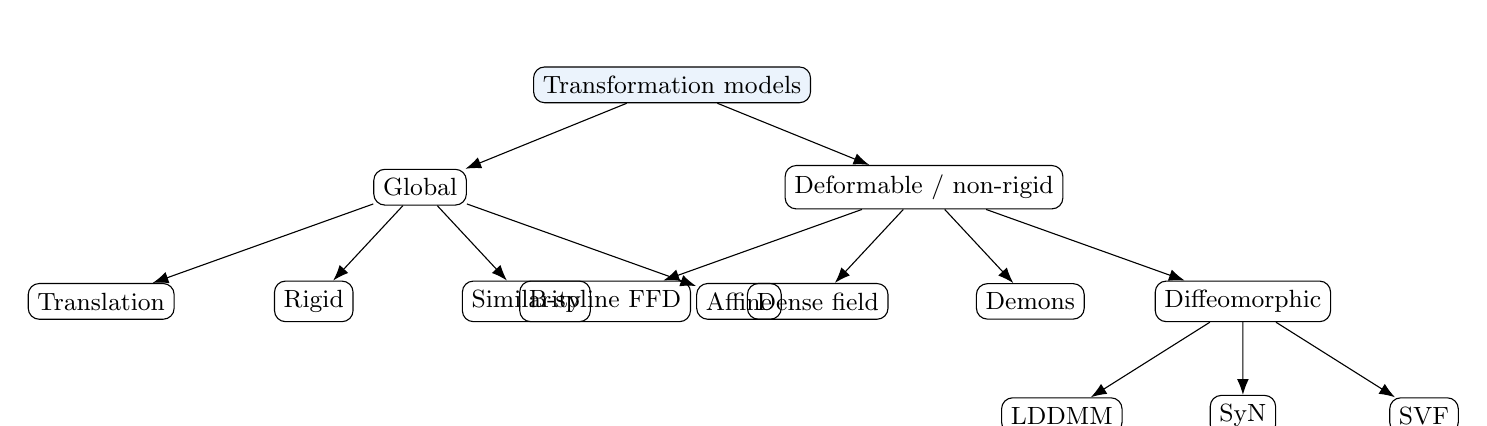
\begin{tikzpicture}[
  every node/.style={draw, rounded corners, align=center, font=\small},
  level 1/.style={sibling distance=6.4cm, level distance=1.3cm},
  level 2/.style={sibling distance=2.7cm, level distance=1.45cm},
  level 3/.style={sibling distance=2.3cm, level distance=1.45cm},
  edge from parent/.style={draw,-{Latex[length=2mm]}}
]
\node[fill=lightblue] {Transformation models}
 child { node {Global}
   child { node {Translation} }
   child { node {Rigid} }
   child { node {Similarity} }
   child { node {Affine} }
 }
 child { node {Deformable / non-rigid}
   child { node {B-spline FFD} }
   child { node {Dense field} }
   child { node {Demons} }
   child { node {Diffeomorphic}
      child { node {LDDMM} }
      child { node {SyN} }
      child { node {SVF} }
   }
 };
\end{tikzpicture}%
}
\end{center}

The important point is that \emph{rotation} and \emph{translation} are low-level components of a global rigid model, while B-splines define a much richer local transformation parameterization.

\section{Worked Example 1: Rigid Surface Registration with ICP}

Assume a moving ultrasound surface contains points $q_i$ and a fixed CT surface contains points $p_j$.

\subsection*{Step 1: Initialization}
Align centroids:
\[
 t_0=\bar p-\bar q.
\]
Set
\[
 T_0(x)=x+t_0.
\]

\subsection*{Step 2: Correspondence Assignment}
For each transformed US point,
\[
 p_i=\argmin_{p\in P}\|T_k(q_i)-p\|.
\]

\subsection*{Step 3: Rigid Solve}
Estimate
\[
(R_{\Delta},t_{\Delta})
=
\argmin_{R,t}\sum_i\|p_i-(RT_k(q_i)+t)\|^2.
\]

\subsection*{Step 4: Transform Composition}
\[
 T_{k+1}=\Delta T_k\circ T_k.
\]

\subsection*{Step 5: Convergence}
Stop when, for example,
\[
|\Loss_{k+1}-\Loss_k|<\epsilon
\]
or the transform update is sufficiently small.

This entire process still produces one global rigid transformation, not one transform per point.

\section{Worked Example 2: Multi-Label SDF Rigid Registration}

Assume five classes:
\[
\mathcal C=\{LV,RV,LA,RA,Myo\}.
\]
For each class, convert fixed and moving masks into normalized SDFs:
\[
\phi_F^c,
\qquad
\phi_M^c.
\]

Choose a rigid transform
\[
T_\theta(x)=R(\theta_x,\theta_y,\theta_z)x+t.
\]

A balanced loss is
\[
\Loss(\theta)
=
\frac{1}{|\mathcal C|}
\sum_{c\in\mathcal C}
\frac{1}{|\Omega_c|}
\sum_{x\in\Omega_c}
\left[
\phi_F^c(x)
-
\phi_M^c(T_\theta^{-1}(x))
\right]^2.
\]

Then solve
\[
\boxed{
\theta^*=\argmin_\theta\Loss(\theta)
}
\]
using a numerical optimizer such as L-BFGS, Powell, or another suitable method.

The resulting six numbers
\[
(\theta_x,\theta_y,\theta_z,t_x,t_y,t_z)
\]
are applied consistently to the entire ultrasound volume and all associated labels.

\section{Worked Example 3: B-Spline Deformable Registration}

Suppose the fixed and moving images are two phases of a cardiac CT sequence. Because the heart changes shape across the cardiac cycle, a rigid transform is insufficient.

Place control points $\Phi_{ijk}$ on a 3D lattice. The displacement field is
\[
 u(x,y,z)
=
\sum_{i,j,k}
B_i(x)B_j(y)B_k(z)\Phi_{ijk}.
\]

The transformation is
\[
T(x)=x+u(x).
\]

An intensity-based objective might be
\[
\Loss(T)
=
-\operatorname{LNCC}\bigl(I_F, I_M\circ T^{-1}\bigr)
+
\lambda\mathcal R(u),
\]
where $\mathcal R(u)$ penalizes non-smooth deformation, for example
\[
\mathcal R(u)
=
\int_\Omega\|\nabla u(x)\|_F^2\,dx.
\]

This is still the same four-layer pattern:
\[
\boxed{
\text{CT intensity}
+
\text{B-spline deformation}
+
\text{LNCC + regularization}
+
\text{numerical optimizer}
}
\]

\section{Application Pattern: Cross-Modal CT--US Followed by CT Phase Propagation}

A useful conceptual pipeline is to separate \emph{cross-modal alignment} from \emph{within-modality cardiac motion}.

First, align a selected 3D ultrasound acquisition to a reference CT phase, for example phase 0:
\[
\boxed{
US
\xrightarrow[\text{SDF / geometry}]{\text{rigid}}
CT_0
}
\]
This is a cross-modal registration problem. The rigid assumption says that the US acquisition is being placed into the CT coordinate system without changing its intrinsic shape.

Second, estimate cardiac motion between CT phases:
\[
CT_0
\xrightarrow{\phi_{0\to t}}
CT_t.
\]
Because cardiac anatomy deforms over time, $\phi_{0\to t}$ is naturally modeled with a deformable transformation such as B-splines, Demons, or a diffeomorphic method.

Once the US image or its labels have been mapped to $CT_0$, they can be propagated through the CT motion field:
\[
US_{CT_0}
\xrightarrow{\phi_{0\to t}}
US_{CT_t}.
\]

Conceptually, therefore,
\[
\boxed{
US
\xrightarrow[\text{cross-modal}]{\text{rigid}}
CT_0
\xrightarrow[\text{intra-modal}]{\text{deformable}}
CT_1,\ldots,CT_{T-1}
}
\]
contains two different registration problems with two different transformation assumptions.

\section{Common Conceptual Mistakes}

\subsection{Mistake 1: ``ICP and SDF are two transformation types.''}

Incorrect. SDF is a representation. ICP is an algorithmic framework. A transformation type would be rigid, affine, B-spline, or diffeomorphic.

\subsection{Mistake 2: ``Each point in rigid ICP gets its own rotation and translation.''}

Incorrect. All correspondences jointly estimate one shared rigid transformation.

\subsection{Mistake 3: ``B-spline is an optimizer.''}

Incorrect. B-spline registration uses a B-spline basis to parameterize a spatially varying deformation field. A separate optimizer is still required.

\subsection{Mistake 4: ``Intensity-based and feature-based are transformation models.''}

Incorrect. They describe the type of information used for registration, so they belong primarily to Layer 1.

\subsection{Mistake 5: ``Rigid registration means ICP.''}

Incorrect. Rigid describes only the transformation model. Rigid registration can be optimized with intensity metrics, SDF losses, landmarks, ICP, or many other methods.

\subsection{Mistake 6: ``If a method gives lower surface distance, it must give better anatomical registration.''}

Not necessarily. A metric can improve while anatomical correspondences become worse. Evaluation should therefore include task-relevant measures such as Dice, ASSD, HD95, landmark error, and qualitative inspection.

\section{Summary Tables}

\subsection{Where Each Concept Belongs}

\begin{longtable}{p{0.34\textwidth}p{0.56\textwidth}}
\toprule
\textbf{Concept} & \textbf{Primary role}\\
\midrule
Raw voxel intensity & Layer 1: representation / signal\\
Binary mask & Layer 1: representation / signal\\
SDF & Layer 1: representation / signal\\
Surface / point cloud & Layer 1: representation / signal\\
Landmark & Layer 1: representation / signal\\
Learned feature map & Layer 1: representation / signal\\
Intensity-based registration & Classification by Layer-1 signal\\
Feature-based registration & Classification by Layer-1 signal\\
Rigid transform & Layer 2: transformation model\\
Rotation / translation & Parameters / primitives inside Layer 2\\
Similarity transform & Layer 2: transformation model\\
Affine transform & Layer 2: transformation model\\
B-spline FFD & Layer 2: transformation model\\
Dense displacement field & Layer 2: transformation model\\
Diffeomorphic transform & Layer 2: transformation model\\
MSE / SSD & Layer 3: objective / metric\\
NCC / LNCC & Layer 3: objective / metric\\
Mutual information & Layer 3: objective / metric\\
Dice & Layer 3: objective / metric\\
SDF difference & Layer 3: objective / metric applied to an SDF representation\\
Chamfer / Hausdorff & Layer 3: geometric objective / metric\\
Adam & Layer 4: optimizer\\
L-BFGS & Layer 4: optimizer\\
Powell & Layer 4: optimizer\\
SVD rigid solve & Layer 4: closed-form solver\\
ICP & Algorithm spanning explicit correspondence, Layer 3 objective, and Layer 4 iterative solving\\
\bottomrule
\end{longtable}

\subsection{Example Registration Pipelines}

\begin{longtable}{p{0.20\textwidth}p{0.20\textwidth}p{0.25\textwidth}p{0.23\textwidth}}
\toprule
\textbf{Representation} & \textbf{Transform} & \textbf{Metric} & \textbf{Solver}\\
\midrule
CT intensity & Rigid & NCC & L-BFGS\\
CT / MRI intensity & Affine & Mutual information & Powell\\
Segmentation masks $\to$ SDF & Rigid & Multi-label SDF loss & L-BFGS / other numerical optimizer\\
Surface points & Rigid & Point-to-point distance & ICP + SVD\\
Surface points + normals & Rigid & Point-to-plane distance & ICP / Gauss--Newton\\
CT intensity & B-spline FFD & LNCC + regularization & L-BFGS / gradient method\\
CT intensity & Diffeomorphic & Image similarity + smoothness & Variational / gradient solver\\
Learned features & Dense field & Feature similarity + regularization & Neural network / gradient optimization\\
\bottomrule
\end{longtable}

\section{A Compact Checklist for Reading Registration Papers}

Whenever a paper says ``we perform registration,'' identify the following explicitly:

\begin{enumerate}
  \item \textbf{Registration signal:} raw intensities, masks, SDFs, landmarks, surfaces, or learned features?
  \item \textbf{Transformation model:} translation, rigid, similarity, affine, B-spline, dense, or diffeomorphic?
  \item \textbf{Parameterization:} Euler angles, quaternions, affine matrix, control-point lattice, displacement field, or velocity field?
  \item \textbf{Similarity / objective:} MSE, NCC, MI, Dice, SDF loss, Chamfer, point-to-plane, or a learned objective?
  \item \textbf{Regularization:} smoothness, bending energy, Jacobian penalty, inverse consistency, topology preservation?
  \item \textbf{Optimization:} SVD, gradient descent, L-BFGS, Gauss--Newton, Powell, alternating optimization, neural inference?
  \item \textbf{Initialization:} identity, centroid alignment, PCA, landmarks, affine pre-registration, previous temporal phase?
  \item \textbf{Evaluation:} Dice, ASSD, HD95, target registration error, landmark error, Jacobian statistics, visual plausibility?
\end{enumerate}

If these eight items are clear, most registration methods become much easier to compare.

\section{Final Mental Model}

The most important conceptual separation is:

\[
\boxed{
\begin{aligned}
\underbrace{\text{What do I match?}}_{\text{Representation}}
&\rightarrow
\underbrace{\text{How may it move?}}_{\text{Transformation}}\\[1mm]
&\rightarrow
\underbrace{\text{How do I score alignment?}}_{\text{Objective}}
\rightarrow
\underbrace{\text{How do I solve it?}}_{\text{Optimizer}}
\end{aligned}
}
\]

Under this model:

\begin{itemize}
  \item \textbf{Intensity-based} and \textbf{feature-based} describe the registration signal.
  \item \textbf{SDF} is a representation derived from a segmentation.
  \item \textbf{Rotation and translation} are primitive parameters of a rigid transformation.
  \item \textbf{B-splines} parameterize a smooth local deformation field.
  \item \textbf{NCC, MI, Dice, SDF loss, Chamfer} are alignment objectives or metrics.
  \item \textbf{Adam, L-BFGS, Powell, Gauss--Newton, SVD} are optimization or solving mechanisms.
  \item \textbf{ICP} is an iterative registration framework that combines explicit nearest-neighbor correspondence estimation with a geometric objective and repeated transform solving.
\end{itemize}

A concise way to describe a method is therefore not simply ``ICP registration'' or ``SDF registration,'' but a full specification such as
\[
\boxed{
\begin{aligned}
&\text{multi-label SDF-based rigid registration}\\
&\text{with balanced SDF loss and L-BFGS optimization}
\end{aligned}
}
\]
or
\[
\boxed{
\begin{aligned}
&\text{label-aware rigid surface ICP with point-to-plane residuals}\\
&\text{and iterative least-squares updates}
\end{aligned}
}
\]

That vocabulary makes the assumptions, degrees of freedom, geometric signal, and optimization procedure explicit.

\end{document}
